\section{Coils}
%\todo{do not link to TU Cloud but instead to the repository!}\\
%\todo{Use \textbackslash{}autoref\{\} instead of \textbackslash{}ref\{\}!}
\subsection{Requirements and Tasks}
The coils should be able to produce a magnetic field of $B = \SI{87}{mT}$ and need to be able to fit into a vacuum-vessel with an inner diameter of $d_o=\SI{1.6}{m}$ and a height of $h=\SI{0.6}{m}$.
The design and optimization team specified that the coil configuration should consist of a total of 12 coils with 3 unique coil types.
The coil configuration provided by the design team should look like Figure \ref{fig:config}.
\begin{figure}[h]
    \centering
    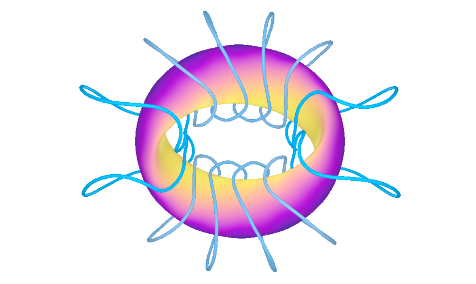
\includegraphics[width=0.5\textwidth]{Images/02_Coils/coil_config.png}
    \caption{Coil configuration- taken from \cite{QUASR}}
    \label{fig:config}
\end{figure}
If possible, the coils should be able to sustain the continuous operation of the Stellarator.
During the cleaning of the vacuum chamber through heating the coils must withstand a temperature of at least $\SI{200}{\degree C}$ for a prolonged period of time.
Furthermore the design of the coils must ensure that the vacuum is not contaminated by any adhesives or materials used.
The generated magnetic field should have a desired deviation from the ideal field of less than \SI{0.2}{\%}.
At last the design must also ensure that the system is collision free, to itself and other elements in the vacuum chamber, and in the realm of manufacturability for a student team.
It follows from these requirements that the coils have to be manufactured very precisely, stiff and robust as well as mounted very precisely within the vacuum chamber.



\subsection{Outcome}
\subsubsection{Structure}
In order to meet the design requirements the overarching structure of a coil is made up of a multitude of water cooled double pancake coils separated by a thin insulator material.
The whole coil structure is then embedded into a steel casing in order to avoid contamination of the vacuum from the used adhesives and material combinations.
%\todo{Sketch of the coil structure - we need to make clear how the product looks like before we describe it in more detail}

\subsubsection{Manufacturing}
It was determined early on that a costly and hard to manufacture solution on the basis of superconductors is not necessary and should be avoided.
Due to the large power losses and the requirement of continuous operation cooling must to be considered.
The most straightforward way of ensuring proper cooling is a water-cooling solution.
To accommodate the water-cooling, the conductor within the coil has to have a hollow cross-section that is big enough to allow for good water flow and heat transport.
Two options to manufacture such a hollow conductor were investigated:
\begin{itemize}
    \item 3D printing the complete coil pack out of copper
    \item Copper pipes bent into the required coil geometries
\end{itemize}
While 3D printers can achieve high purity prints, with effective conductivities being close to 99\% of pure copper, current manufacturing methods do not allow us to print the geometries in the necessary dimensions and with a suitable internal surface smoothness.
The internal roughness is of special concern, since water has to flow through the windings without too much pressure loss.
Additionally the powder used during manufacturing remains in the channels and can be difficult do remove from the manufactured coils.
Due to this it was decided to use conventional manufacturing methods.
While the manufacturing of the complex geometries might prove challenging for future teams the advantages of off the shelf copper conductors, especially high performance conductors, cannot be overstated.
As mentioned above the coils are designed to be inside a casing, which addresses both outgassing concerns, a well as the feedthroughs for water and current.
For the casing of the coils, electron beam sintering could be considered in addition to 5-axis milling in order to achieve the necessary accuracy.
The casings are flanged to the walls of the vacuum chamber, such that the inside of the casings are not under vacuum, which makes the design of the winding pack easier.\\
(for more: \href{https://cloud.tugraz.at/index.php/apps/onlyoffice/s/XBeMB6XiRDt3L2p?fileId=1032740140}{"Isolation and 3D Printing" Powerpoint presentation}).

\subsubsection{Insulation}
The windings within a coil have to be insulated from each other.
The best option seems to be fibre glass reinforced epoxy, as it be bought in pre-impregnated rolls and further improves stability.
The epoxy has to be hardened for which the coil might have to cooled, using the already in place water-cooling.
However, then the epoxy can withstand the applied temperature and forces and it should be around \SI{0.5}{mm} to \SI{1.0}{mm} thick.
In order to prevent outgassing of the coils into the vacuum chamber, they are to be enclosed with a stainless steel casing of \SI{2.0}{mm} thickness, which could either be 3D printed or manufactured by arc welding sheet metal.\\

\subsubsection{Optimization}
A python script was developed in order to explore the space of possible configurations.
In the beginning rough estimates for the magnetic field and size were used, they were later replaced by the actual currents supplied by the optimization team and the size of the vacuum chamber.
The overall goal was to reduce both power loss and pressure loss, while staying within some reasonable bounds for voltage and current.
This was done for different winding configurations and pipe diameters.
Figure \ref{fig:both} shows an example output. The simulation is based on double pancakes, meaning, that two neighbouring coils are paired and supplied with water separately.
\begin{figure}[h]
    \centering
    \begin{subfigure}[b]{0.7\textwidth}
        \centering
        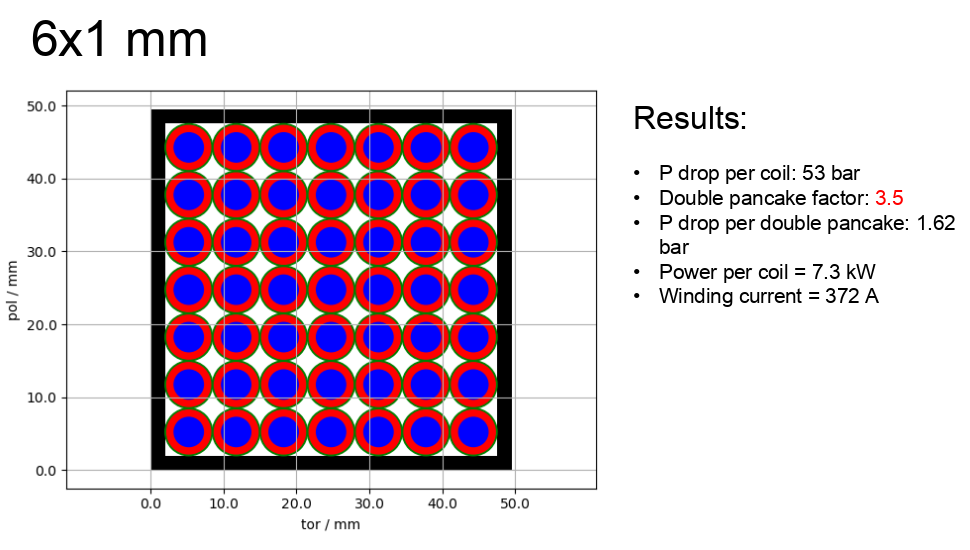
\includegraphics[width=\textwidth]{Images/02_Coils/crosssection.png}
        \caption{Coil cross-section of 7x7 windings.}
        \label{fig:crosssection}
    \end{subfigure}\hfill
    \begin{subfigure}[b]{0.3\textwidth}
        \centering
        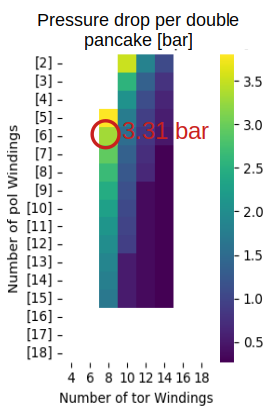
\includegraphics[width=0.9\textwidth]{Images/02_Coils/pressure.png}
        \caption{pressure drop}
        \label{fig:pressure}
    \end{subfigure}
    \caption{6x1mm pipe configuration and 6x1mm pipe pressure drop calculation for different configurations}
    \label{fig:both}
\end{figure}

A design with rectangular pipes and circular holes for water, greatly improves the power loss and pressure loss characteristics. %\todo{Where is an image of it?@Mimo please run the simulation for conductors with the square outer cross section that we can display it}
While these pipes exist and a re-used for high current applications, it is unclear if there are suppliers which could be contacted. %\todo{Cite Luvato and the sketchy supplier}\\
(for more see \href{https://github.com/LiigaSoolane/coil}{Github})\\
In order to validate these results an experiment was designed.
However, due to problems with the delivery of equipment, the test has not yet been conducted.\\
\subsubsection{3D Modeling}
The filaments, created by the optimization team have been imported into fusion 360, however the program was not able to process the actual extrusion process, as especially constructed coordinate systems had to be used in order to ensure the coils not touching.
For this purpose Python and CadQuery were used. %\todo{citation of CadQuery}
Furthermore, Python scripts for the determination of the maximum dimension as well as the minimum distance between coil filaments were created.
This was then also used to determine the scaling factor for the optimization teams data (it was set to be 0.33).
Due to collisions of the coil, the final coil cross-section was set to (40x67)~mm.\\

%\textcolor{red}{Daniel: Add pictures of the coils model}

A mount for the coils was conceptually drawn and constructed in Autodesk Fusion as can be seen in figure \ref{fig:mount}.
It enables the coils to be mounted to the vacuum chamber and to be adjusted and aligned them from outside the chamber.
Additionally it serves as port for the electrical cables and the water hoses.
In order to allow for movement through the walls of the vacuum chamber a bellow has to be used.
%\todo{The drawing should use the same colors as the crosssection on the left}
\begin{figure}[H]
    \begin{subfigure}[b]{0.5\textwidth}
        \centering
        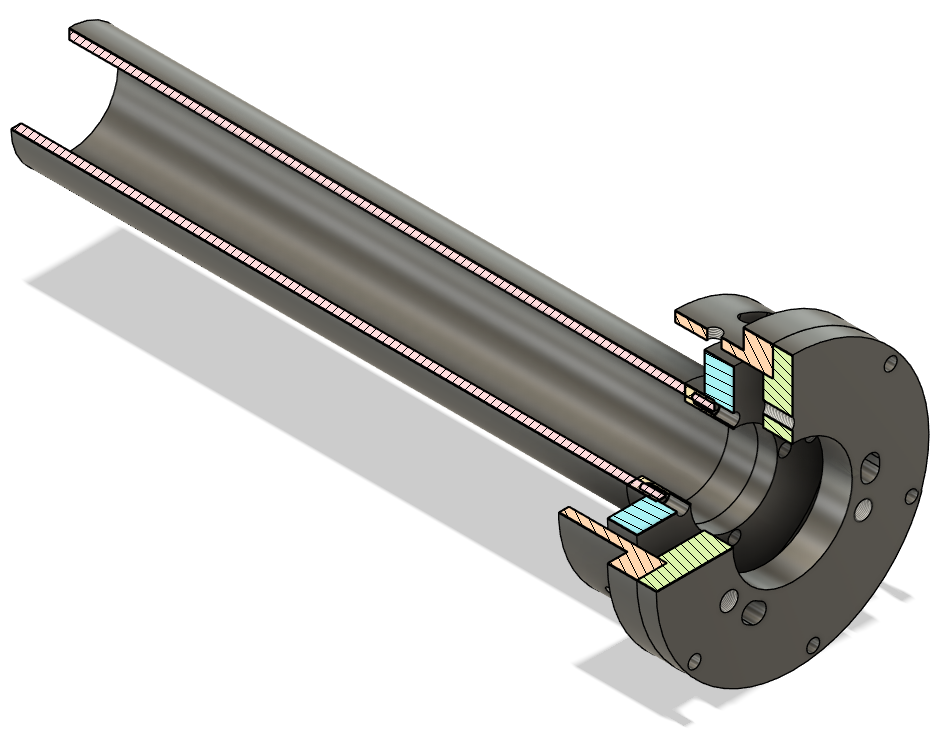
\includegraphics[width=\textwidth]{Images/02_Coils/Coil_mount_crosssection.png}
        \label{fig:Coil mount crosssection}
    \end{subfigure}
    \hfill
    \begin{subfigure}[b]{0.5\textwidth}
        \centering
        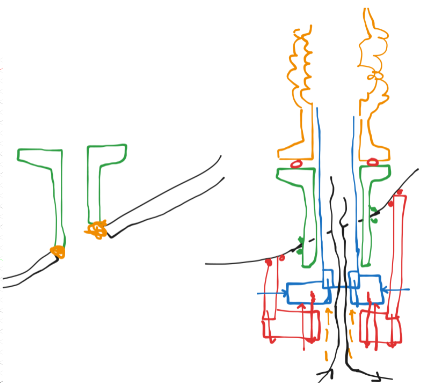
\includegraphics[width=\textwidth]{Images/02_Coils/coil_mount.png}
        \label{fig:Coil mount drawing}
    \end{subfigure}
    \caption{Coil Mount and principle. The left picture shows the modelled manipulator, which allows for precise alignment of the coils. The right pictures show a sketch of the attachment scheme.}
    \label{fig:mount}
\end{figure}
To calculate both magnetic fields and Lorentz forces between coils, another python script was written.
It also enable the calculations of moments, in the center of mass of the coils.
The forces due to the magnetic fields were found to be much weaker than the ones due to gravity, which is why it was decided to mount the coils directly over there center of gravity, without any additional reinforcement.
Figure \ref{fig:mount_stress} shows the deformation due the expected forces along the mounting mechanism.
\begin{figure}[H]
    \centering
    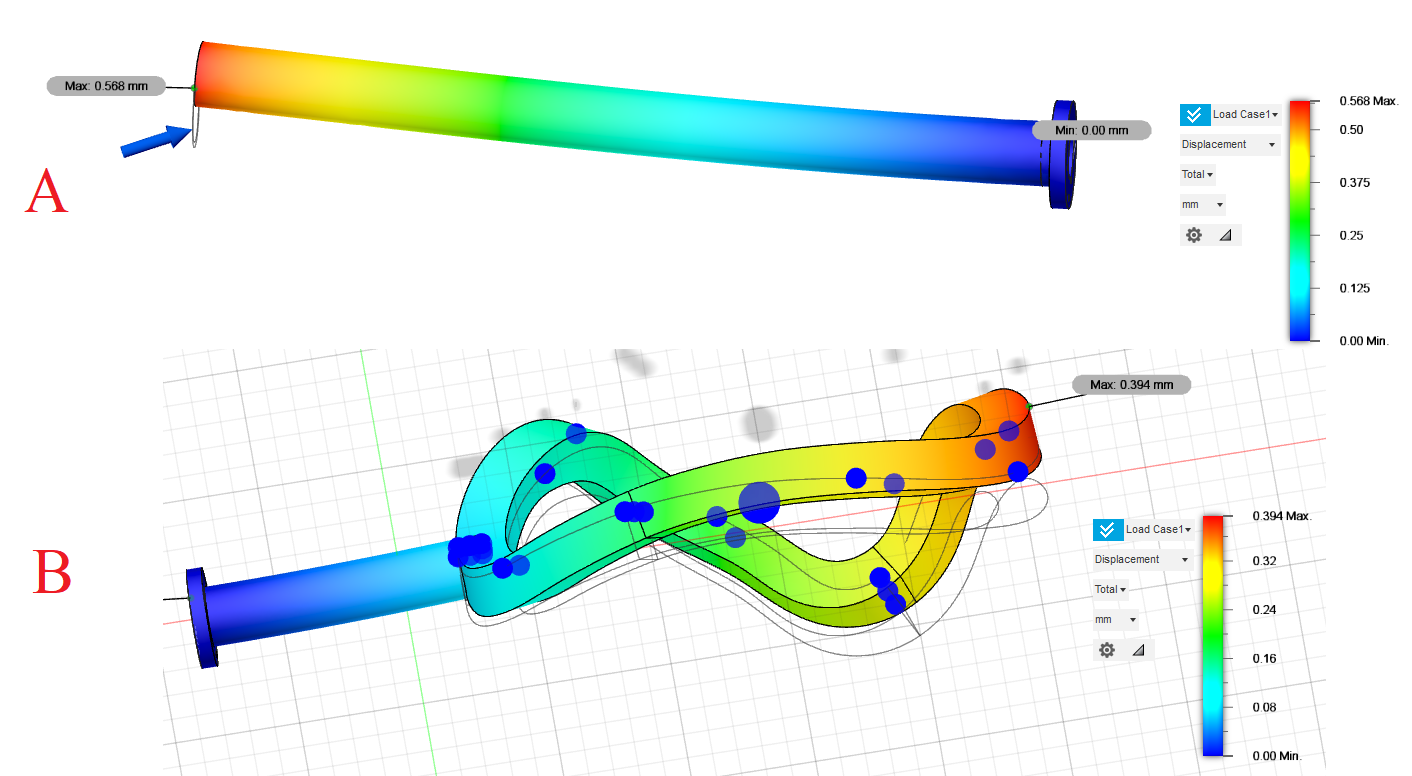
\includegraphics[width=0.7\textwidth]{Images/02_Coils/mount_stress.png}
    \caption{A: the deformation of a steel tube with \SI{80}{cm} (approximated distance of coil center of mass to attachment point). B: the deformation of a full coil model, with forces still acting in the center of mass.}
    \label{fig:mount_stress}
\end{figure}

% \subsection{Required Materials}
% \todo{Jonathan: shopping}

% required support facilities?
% power supplies - total required power, targeted voltage, targeted current, ... - does it work with HP/Agilent N8951A?
% water cooling - required flow, pressure, deposited power, ...
% instrumentation: water flow sensors, current sensors, ...

% required parts list ("Bill of Materials")
% 2 or 3 double pancakes per coil, each 16 (2x8) windings
% 2 coil casing halves per coil
% feedthroughs for chamber flanges
% vacuum bellows, clamps, O-ring seals


\subsection{Outlook}
The following points can be seen as next steps:
\begin{itemize}
    \item The experimental verification of the design space model has to be completed.
    \item The manufacturing process of the coils has to be examined in greater detail.
    \item Further detailing of the CAD models has to be done.
    \item The magnetic and structural behaviour of the coils should be validated via detailed Multiphysics FEM simulation. This simulation has to take in account that the coils are essentially composites with an inhomogeneous and anisotropic behaviour.
    \item Further refining of the CAD Model and creation of 2D drawings for manufacturing.
\end{itemize}

\subsection{Learnings}
One big revelation is how difficult it is to draw the CAD Model and that Fusion 360 is not capable of such complex operations.
This comes from the complicated filament geometry.
Another challenge was to model the transition between each winding.
One of the bigger challenges connected to this was to find a local coordinate system for which the coils do not collide and also do not deform too much.

% * simulation
% * double pancake concept - factor
% * highly non-linear pressure drop - large gains from routing water channels in parallel
% * square conductor with round bore - extremely high performance, makes everything better

% * choice of local coordinate system in individual segments of filament - tricky
% * found ways to align coil shape in this - avoid coil collisions

% * stabilizing of individual windings during manufacturing: epoxy/fibre-glass mix to make sure windings stay in place
% * forces on windings: Lorentz + gravity; Lorentz not dominant(?) wrt. gravity
% * outgassing: coils need to be enclosed in stainless steel casing
% * feed-throughs: can expose inside of coil casing to outer world
% * via bellow allows online adjustment of coil positions
% * locally stitch windings together




